
%(BEGIN_QUESTION)
% Copyright 2014, Tony R. Kuphaldt, released under the Creative Commons Attribution License (v 1.0)
% This means you may do almost anything with this work of mine, so long as you give me proper credit

Calculate all voltages and all currents in this transformer circuit, assuming a load current of 31 mA:

$$\includegraphics[width=15.5cm]{i01266x01.eps}$$

\begin{itemize}
\item{} $V_{primary}$ = 
\item{} $V_{secondary}$ = 
\item{} $I_{primary}$ = 
\item{} $I_{secondary}$ = 
\end{itemize}

\vfil 

\underbar{file i01266}
\eject
%(END_QUESTION)





%(BEGIN_ANSWER)

This is a graded question -- no answers or hints given!

%(END_ANSWER)





%(BEGIN_NOTES)

\begin{itemize}
\item{} $V_{primary}$ = 83.3 volts
\item{} $V_{secondary}$ = 15.19 volts
\item{} $I_{primary}$ = 5.653 milliamps
\item{} $I_{secondary}$ = 31 milliamps
\end{itemize}

A good way to check your work with transformer calculations is to take your voltage and current values and use them to calculate {\it power} for both the primary winding and the secondary winding.  For an ideal power transformer these input and output power values must be precisely equal in accordance with the Law of Energy Conservation.

%INDEX% Electronics review: transformer ratios

%(END_NOTES)


